\documentclass[tikz]{standalone}
\usetikzlibrary{datavisualization}
\usetikzlibrary{datavisualization.formats.functions}
\begin{document}
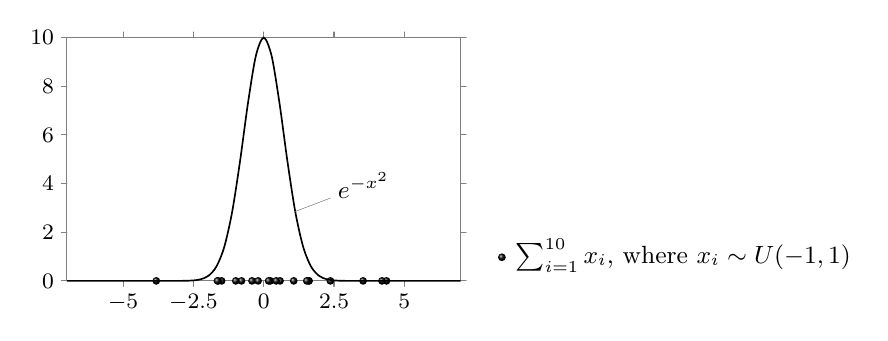
\begin{tikzpicture}
\datavisualization [scientific axes]
[
visualize as smooth line=Gaussian,
Gaussian={pin in data={text={$e^{-x^2}$},when=x is 1}}
]
data [format=function] {
	var x : interval [-7:7] samples 51;
	func y = 10*exp(-\value x*\value x);
}
[
visualize as scatter,
legend={south east outside},
scatter={
  %style={mark=*,mark size=1.4pt},
  style={mark=ball,ball color=black,mark size=1.4pt},
  label in legend={text={
  	$\sum_{i=1}^{10} x_i$, where $x_i \sim U(-1,1) $}}}
  	]
data [format=function] {
	var i : interval [0:1] samples 20;
	func y = 0;
	func x = (rand + rand + rand + rand + rand +
	rand + rand + rand + rand + rand);
};
\end{tikzpicture}
\end{document}
